\section{Ausreißer und Ähnlichkeit}
In diesem Abschnitt folgen die Erklärungen der Begriffe Ausreißer und Ähnlichkeit, im Kontext von Zeitreihen.
\subsection{Ausreißer}
Ane Blázquez"=García et al. \cite[Ch. 2.2]{reviewOutlierDetection} unterscheiden drei verschiedene Typen von Ausreißern. Darunter zählen Punkt"=Ausreißer (engl. \textit{Point outliers}), Teilfolge"=Ausreißer (engl. \textit{Subsequence outliers}) und Zeitreihen"=Ausreißer (engl. \textit{Outlier time series}).

Ein Punkt"=Ausreißer ist ein einzelner Datenpunkt, der, verglichen mit anderen Datenpunkten, auffällig anders ist. Dabei unterscheidet man zwischen einem lokalen und einem globalen Punkt"=Ausreißer, je nachdem, ob man nur mit Punkten in einem gewissen Abstand zum Referenzpunkt (lokal) oder mit allen Punkten der Zeitreihe (global) vergleicht.

Ein Teilfolge"=Ausreißer besteht aus aufeinanderfolgende Datenpunkten, die, verglichen mit anderen Teilfolgen, auffällig anders sind. Dabei müssen die einzelnen Punkte nicht zwanghaft Punkt"=Ausreißer sein, sondern die Folge in ihrer Gänze muss auffällig sein. 

Der für diese Arbeit relevante Typ ist der Zeitreihen"=Ausreißer. Bei diesem Typ ist das Verhalten einer kompletten Zeitreihe, verglichen mit anderen Zeitreihen, auffällig anders. In der Definition vom oben erwähnten Paper \cite{reviewOutlierDetection} ist außerdem die Rede davon, dass die Zeitreihe eine multivariate sein muss, um Zeitreihen"=Ausreißer zu erkennen, denn mit nur einer Reihe an Werten kann kein Vergleich zwischen mehreren Reihen gemacht werden. Diese Bedingung schließt allerdings nicht aus, mehrere \acs{UZR} mit gleicher Länge und gleichem Messintervall zu einer gemeinsamen \acs{MZR} zusammenzuführen. In \autoref{fig:ZeitreihenAusreisserBeispiel} ist eine an \cite[Fig. 5]{reviewOutlierDetection} angelehnte Abbildung einer \acs{MZR} zu finden, die mit Variable 4 ein Beispiel für einen Zeitreihen"=Ausreißer zeigt.
\begin{figure}[bth] 
  \centering
  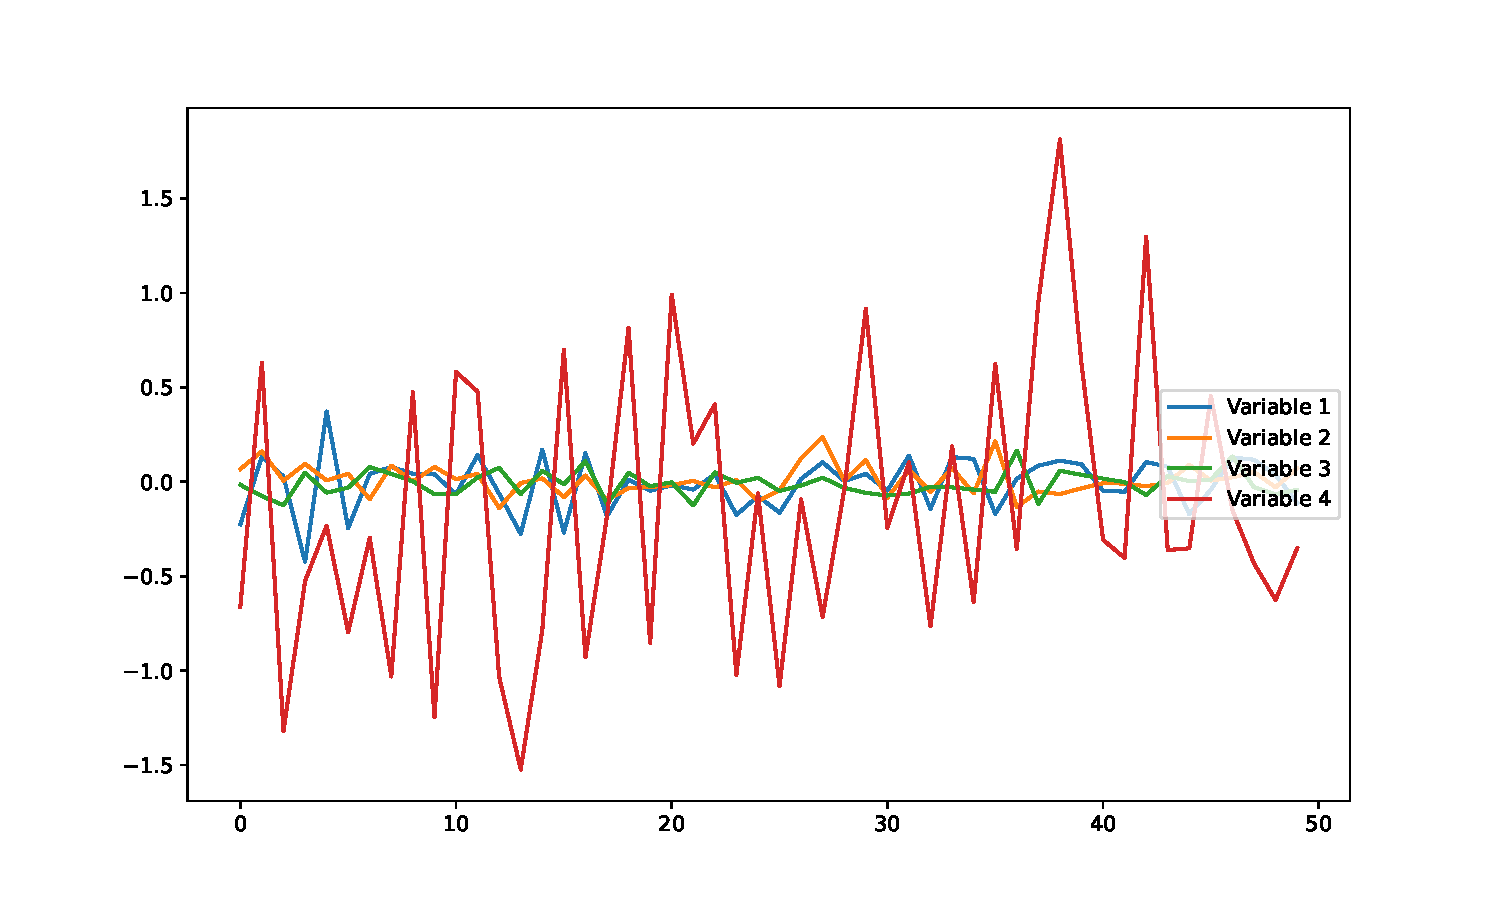
\includegraphics[width=0.7\textwidth]{Graphics/TimeSeriesOutlierExample.pdf}
  \caption{Zeitreihen"=Ausreißer (Variable 4) in einer \acs{MZR}}
  \label{fig:ZeitreihenAusreisserBeispiel}
\end{figure}

\subsection{Ähnlichkeit}\label{subsec:aehnlichkeit}
Ähnlichkeit oder genauer die Ähnlichkeitssuche wird in "`Billion-Scale Similarity Search with GPUs"' \cite[Ch. 2]{faissAehnlichkeitssuche} folgendermaßen beschrieben: Gegeben sei ein Beispielvektor $x \in \mathbb{R}^d$ und eine Ansammlung von Vektoren $[y_0,y_1,\ldots,y_{n-1}]$ mit $y_i \in \mathbb{R}^d$. Ziel ist es, die Menge $L$ mit den Indizes der $k$ Elemente aus der Ansammlung zu finden, die die kleinste Euklidische Distanz zu $x$ haben. Die Menge $L$ kann also mit
\[L= k \text{-}\argmin_{i=0,\ldots,n-1}\|x-y_i\|_2\]
beschrieben werden. Dabei wird mittels $\|x-y_i\|_2$ die Euklidische"=Distanz \\ $\|x-y_i\|_2=\|v\|_2 = (v_0^2+v_1^2+ \ldots +v_{n-1}^2)^{1/2}$ berechnet, und es werden mittels  des Ausdrucks $k\text{-}\argmin_{i=0,\ldots,n-1}$ die $k$ Indizes der $k$ kleinsten enthaltenen Werte ausgewählt.

Im Kontext unserer Zeitreihen ist der Vektor $x$ eine Repräsentation einer Zeitreihe, zu der wir die nächsten Nachbarn finden möchten, und alle übrigen Zeitreihen gehören zu der Ansammlung, mit der verglichen wird.